\section{Behavior tree nodes}
    Here we will present the implementation of individual nodes in our algorithm. We will split the nodes into categories based on the sub-tree they belong to. We will also show the basic functionality of the library used.
    \subsection{Introduction}
        The BT algorithm is implemented using the behaviortree-cpp-v3 library. Therefore, we will present how we create, implement and start polling the tree. We will also show how nodes are created, implemented, and used.\\\\
        \bfc{Creating the node}\\
            To create the node, we need to create a class that inherits from one of the parent classes in the library. The parent classes depend on the type of node we want to create. If we create an action node, we inherit from the \texttt{SyncActionNode} class. If we create a condition node, we will inherit from the \texttt{ConditionNode} class.\\
            There are two mandatory functions for all nodes, the \texttt{tick} and \texttt{providedPorts} functions. These two functions must be implemented, or an error will occur.\\
            The \texttt{tick} function is responsible for the actual implementation of the node. It is called every time the node is polled. It is also responsible for returning the state of the node.\\
            The \texttt{providedPorts} function defines the ports the node will use. This function must be defined even if the node does not use any ports.\\\\
        \bfc{Using the node}\\
            To use a node, we must register it in the \texttt{BehaviorTreeFactory} object. We do this by calling the \texttt{registerNodeType} function. For this function, we need to specify the class of the node we want to register, e.g., one of the nodes we created. It also takes one \texttt{std::string} parameter, which identifies the name of the node in our BT algorithm \texttt{.xml} file.\\\\
        \bfc{Creating and running the tree}\\
            To create the tree, we first must have a \texttt{.xml} file with the tree structure. This file is then parsed by the \texttt{BehaviorTreeFactory} object using the \texttt{createTreeFromFile} function. The result is a \texttt{Tree} object which we can store and later run. Ahead of calling the parsing for the tree file, all the nodes used in the file must be registered.\\
            To run the tree, we call the \texttt{tickRoot} function on the \texttt{Tree} object. This function returns the state of the root node of the tree.\\\\
        \bfc{Blackboard}\\
            The blackboard is a shared memory between the nodes of the tree. It is used to store data that is being utilized by multiple nodes.\\
            It is also the reason why we implement the \texttt{providedPorts} function. This function specifies the ports the node will use. The ports can serve as an \texttt{input}, an \texttt{output}, or both. \texttt{Input} ports can take a constant value (specified in the \texttt{.xml} file of the tree structure) or look for a value in the blackboard.\\\\
        \bfc{Logging}\\
            The BT library also provides us with logging functionality. This functionality is useful for debugging and testing.\\
            We can use different types of loggers. The most common one is the \texttt{StdCoutLogger} which logs to the standard output. We can also use the \texttt{FileLogger}, which saves logs to a file.\\
            We will use the \texttt{FileLogger} to log the tree execution. This logger is useful for its integration with the \texttt{Groot} application as we can import the produced file and visualize the polling of our BT structure.\\
            The logging will be used only for debugging and testing purposes and serves no other function in the final product.
    \subsection{Main BT}
        In this BT, we only have one non-sub-tree node. This is because this sub-tree encodes the algorithm's structure rather than having nodes for execution.\\\\
        \bfc{StartAlgorithm -- Condition node}\\
            This node is responsible for determining whether the robot is in the phase of crossing the road during its mission. It is necessary to implement such a node to facilitate the transfer of control from path planning to road crossing. In contrast, we could determine if the crossing should start based on the distance of the robot from the road. However, this method would fail whenever our robot has to walk alongside any road.\\
            This node is implemented as a ROS service updating a static variable, which is checked when the node is ticked.\\
            This service should be used mainly by other nodes outside of the package itself, with one notable exception. The exception being the very last node of our tree. It serves as a prevention against the looping of our algorithm.
    \subsection{Init BT}
\label{sec:Init-BT-impl}
    Here we will present the nodes used in the Init sub-tree. This sub-tree is used to initialize the BT algorithm. It is the first sub-tree to be executed. This tree is going to be executed only once per road crossing.\\\\
    \bfc{GetPosition -- Action node}\\
        This node is responsible for obtaining the current GPS position of the robot and converting it to the UTM coordinate system. It is implemented as a ROS topic subscriber. The topic subscribed is \texttt{/gps/fix} where the GPS data are being published.\\
        The obtained data are then converted to UTM using the \texttt{gps\_to\_utm} function defined in \ref{sec:geo_func}. The result is then stored as two BT blackboard variables -- \texttt{easting} and \texttt{northing}.\\
        For every obtained value, it also calls a ROS service \texttt{place\_suitability} to determine the suitability of the current position for crossing.\\\\
    \bfc{CrossRoad -- Condition node}\\
        This node tells our algorithm if we are close enough to a road to take over the robot's controls. If we are not the path-planning or other node is left in control.\\
        We use the return values of the ROS service call issued in the \texttt{GetPosition} node. This service has two return values -- \texttt{validity} and \texttt{suitability}. \texttt{Suitability} uses the road cost as well as context score to judge the place for crossing. For \texttt{validity}, we only calculate the distance of the current location to road segments from OSM.\\
        Therefore the \texttt{validity} variable is the one determining the output of this node. The distance limit we proposed as sufficient is $10\:\rm{m}$ from the center of the road.\\\\
    \bfc{PlaceSuitable -- Condition node}\\
        This node states whether the current robot's location, stored as a blackboard variable, is suitable for crossing.\\
        It uses the second return value from the ROS service called in the \texttt{GetPosition} node. As stated, this value takes into account the road cost for our location from the road-cost algorithm (\ref{sec:road_cost}) and the context score calculated separately before the service call.\\
        The context score is based on the contextual information that is available to us. This information may be passed from other nodes (e.g., computer vision node for detecting road parameters) or set by the operator.\\
        The calculation of the context score and the process of obtaining the contextual information is described in \ref{sec:context}.\\\\

    \noindent Other nodes shown it the BT structure (fig \ref{fig:Init-BT}) are currently returning \texttt{FAILURE}. These nodes are there to show the potential for further work. Their main purpose is to steer the robot to a more optimal location for crossing. In this work, we assume that the correct location was chosen in the pre-mission planning.
    \subsection{Perpendicular BT}
\label{sec:Perpendicular-BT-impl}
    The task of this tree is to position the robot perpendicular to the road. It is the second sub-tree to be executed, and as well as Init BT, it is used to prepare the robot for the crossing and is only executed once.\\\\
    \bfc{GetAzimuth -- action node}\\
        This node is responsible for obtaining the robot's current azimuth. We have a ROS subscriber listening to topic published by \texttt{compass} node\footnote{\url{https://github.com/ctu-vras/compass}}.\\
        The compass node may publish the azimuth in several different formats. In our program, we use the ENU format in radians. But if the compass node publishes the azimuth in a different format, we have subscribers that can convert it to the desired format.\\
        The azimuth is then stored as a blackboard variable \texttt{azimuth}.\\\\
    \bfc{RoadHeading -- action node}\\
        This node calculates the heading of the closest road to the robot. We take the current robot's position from the blackboard variable \texttt{easting} and \texttt{northing} and send a request to the ROS service \texttt{get\_road\_heading}.\\
        The service returns the two coordinate points representing the closest road segment's starting and ending points.\\
        We then calculate the heading of the road segment using the function defined in section \ref{sec:geo_func}.\\
        The calculated road heading is then stored as a blackboard variable \texttt{road\_heading}.\\\\
    \bfc{ComputeHeading -- action node}\\
        This node uses the blackboard variable \texttt{azimuth} and \texttt{road\_heading} to calculate the heading the robot should achieve to be perpendicular to the road.\\
        The calculation is defined in section \ref{sec:geo_func}.\\
        The result is stored as a blackboard variable \texttt{req\_azimuth}.\\\\
    \bfc{RobotPerpendicular -- condition node}\\
        This node checks if the robot is perpendicular to the road. It works by comparing the current azimuth with the required heading. Both of these values are stored in the blackboard.\\
        We use the function defined in section \ref{sec:math_func} to compare the values to calculate the difference between two angles. The result is then compared to the threshold value, which is set to $0.1745\:\rm{rad}$ or $10\rm{^{\circ}}$.\\\\
    \bfc{RotateRobot -- action node}\\
        This node rotates the robot to the required heading.\\
        First, we calculate the difference between the robot's current and desired azimuth. Then, based on the difference, we proportionally set the rotation direction and speed.\\
        The calculated movement is then published to the \texttt{cmd\_vel} topic.\\\\
    \bfc{StepFromRoad -- action node}\\
        If, for whatever reason, the robot is not able to rotate safely, primarily due to the possibility of ending on the road, we use this node to move the robot away from the road.\\
        Firstly we check the difference between the robot's current azimuth and the road heading. Based on the difference, we set the direction of the movement.\\
        The movement is then published to the \texttt{cmd\_vel} topic.

    \subsection{Crossing BT}
\label{sec:Crossing-BT-impl}
    This tree is used for the main decision-making process. It is the third sub-tree to be executed, and the only one to be executed repeatedly.\\
    In multiple nodes we will use information about the detected vehicles, and collision parameters for each vehicle. Therefore, we first need to define the data structures used to store this information.\\\\
    \bfc{Vehicle data}\\
        The data structure for storing the information about the detected vehicles is defined as follows:
        \begin{lstlisting}[language=C++, caption={Vehicle data structure}, label={lst:vehicle_data}]
            struct vehicle_info {
                int id;
                double x_pos;
                double y_pos;
                double x_dot;
                double y_dot;
                double x_ddot;
                double y_ddot;
                double length;
                double width;
            };
            struct vehicles_data {
                int num_vehicles;
                std::vector<vehicle_info> data;
            };
        \end{lstlisting}
        The first struct \texttt{vehicle\_info} is used to store the information about single detected vehicle. The position of the vehicle is expressed in relation to the robot's frame. The robot frame means, the center of the robot is the origin of the coordinate system. The $x$-axis points forward from robot and the $y$-axis points to the left.\\
        The second struct \texttt{vehicles\_data} is used to store the \texttt{vehicle\_info} structs of all detected vehicles.\\\\
    \bfc{Collision data}\\
        The data structure for storing the collision parameters has the following definition:
        \begin{lstlisting}[language=C++, caption={Collision data structure}, label={lst:collision_data}]
            struct collision_info {
                int car_id;
                double v_front;
                double v_back;
                bool collide;
                bool collide_stop;
            };
            struct collisions_data {
                int num_collisions;
                std::vector<collision_info> data;
            };
        \end{lstlisting}
        The first struct \texttt{collision\_data} is used to store the collision parameters for single vehicle.\\
        The \texttt{v\_front} and \texttt{v\_back} variables are the velocities of the robot to come into contact with the front or back of the vehicle. The figure \ref{fig:collision} shows the contact points we are calculating the velocities for. The figure is explained in the next part.\\
        The \texttt{collide} variable is a boolean value that tells us if the robot is going to collide with the vehicle. It is calculated based on the current velocities of the robot and the vehicle.\\
        The second struct \texttt{collisions\_data} is used to store the information about collisions with all detected vehicles.\\\\
    \bfc{Used units}\\
        We use these units for the measured and calculated parameters:
        \begin{itemize}
            \item \textbf{Position} -- meters $[\rm{m}]$
            \item \textbf{Time} -- seconds $[\rm{s}]$
            \item \textbf{Velocity} -- meters per second $[\rm{m\,s^{-1}}]$
            \item \textbf{Acceleration} -- meters per second squared $[\rm{m\,s^{-2}}]$
            \item \textbf{Dimensions} -- meters $[\rm{m}]$
        \end{itemize}
    \bfc{Calculating the collision parameters}\\
        First, we need to state the assumptions we are making in order to simplify the calculation.\\
        The first assumption is about the coordinate system we are using. We are using the robot's frame, where the robot's center is the system's origin, and all the positions are expressed in relation to this origin. The $x$-axis points forward, and the $y$-axis points to the left. We can assume this because the calculations are done periodically, and the results are only relevant for the current time step. It also simplifies the process, as the vehicle positions are already expressed in the robot frame.\\
        The second assumption is about the movement of the robot. We assume the robot is moving in a straight line with constant velocity. This is reasonable as we want the robot to be as predictable as possible, so we do not want to move the robot to the side. The assumption about the constant velocity, meaning the acceleration is zero, is also reasonable. The speeds the robot can achieve are much lower than the robot's acceleration, we can therefore neglect the acceleration.\\
        The third assumption is about the movement of the vehicle. We assume the vehicle's acceleration is constant. This is a reasonable simplification as the calculation is done periodically.\\
        The fourth assumption is that we will calculate the collision only in two dimensions. This is reasonable as the $z$-axis will not impact the occurance of a collision. Moreover, the area over which the collision can occur is relatively small, and therefore, any terrain deviation will not impact the collision significantly.\\\\
        Figure \ref{fig:collision} depicts a schematic view of the collision. There are two contact points, both on the robot and the vehicle. The first one (blue) is the point where the robot is going to collide with the front of the vehicle. The second one (red) is the point where the robot is going to collide with the back of the vehicle.\\
        \begin{figure}[ht]
            \centering
            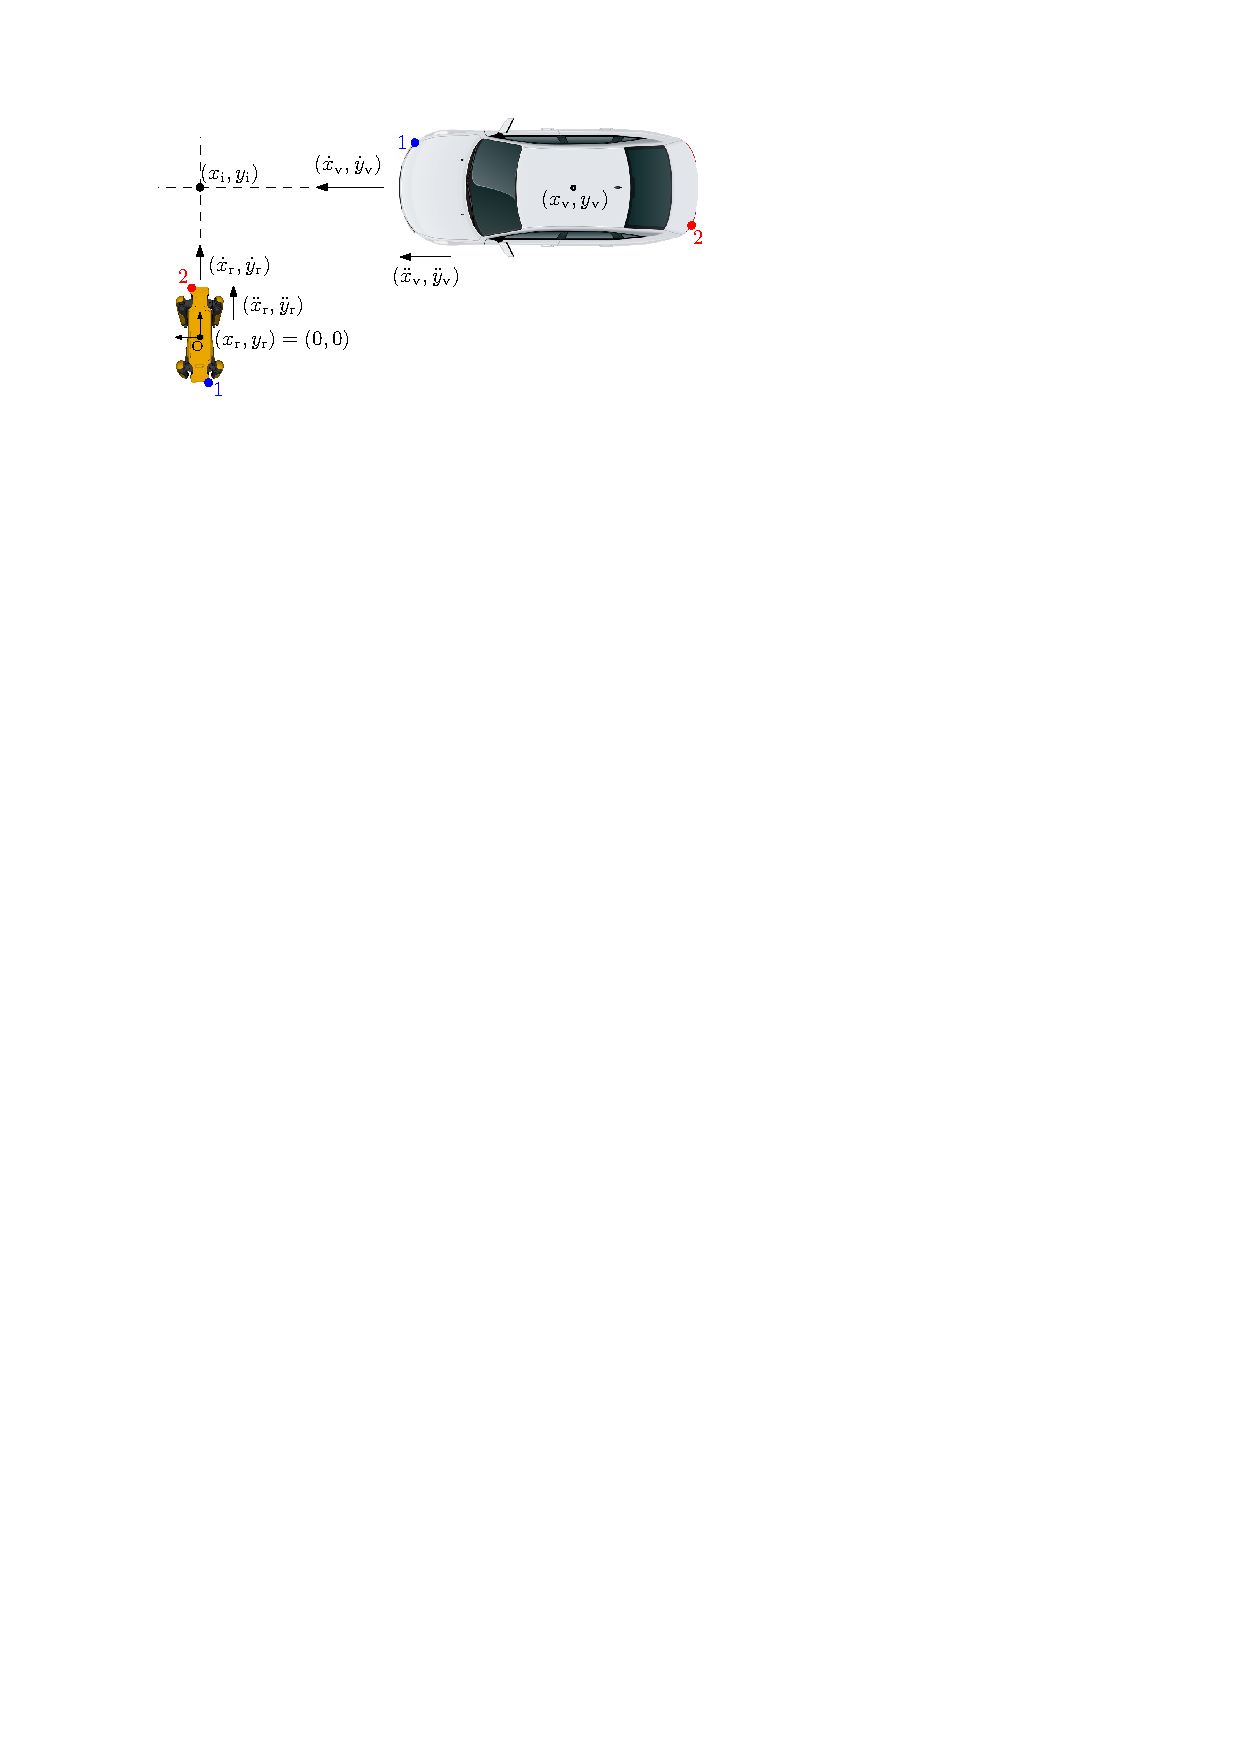
\includegraphics[height=6cm]{images/collision.pdf}
            \caption{Visualization of collision points, coordinate system, and vehicle parameters.}
            \label{fig:collision}
        \end{figure}
        \noindent For the first point, we calculate the velocity \texttt{v\_front}. This velocity depicts the minimal speed of the robot to cross in front of the vehicle. We calculate the velocity \texttt{v\_back} for the second point. This velocity depicts the maximal speed of the robot to cross behind the vehicle.\\
        The subscript \texttt{r} is used for parameters of the robot, and the subscript \texttt{v} is used for parameters of the vehicle.\\
        The calculation is divided into three parts. In the first part, we determine the starting positions of the robot and the vehicle. In the second part, we calculate the time when the vehicle will reach the intersection point $(x_{\rm{i}}, y_{\rm{i}})$. In the last part, we calculate the velocities for the robot to collide with the vehicle.\\\\
        The first part is necessary as the coordinates of both the robot and the vehicle are at the center of their respective bodies. We need to move the starting points concerning the robot's and vehicle's length and width. The starting points for the robot are calculated using these equations:
        \begin{align}
            x_{\rm{r,f}} &= \frac{l_{\rm{r}}+w_{\rm{v}}}{2},\\
            x_{\rm{r,b}} &= -\frac{l_{\rm{r}}+w_{\rm{v}}}{2},\\
            y_{\rm{r,f}} &= y_{\rm{r,b}} = 0,
        \end{align}
        where $l_{\rm{r}}$ is the length of the robot and $w_{\rm{v}}$ is the width of the vehicle.\\
        The starting points for the vehicle are calculated as follows:
        \begin{align}
            x_{\rm{v,f}} &= x_{\rm{v}} + \frac{l_{\rm{v}}+w_{\rm{r}}}{2}\cos{(\varphi_{\rm{v}})},\\
            x_{\rm{v,b}} &= x_{\rm{v}} - \frac{l_{\rm{v}}+w_{\rm{r}}}{2}\cos{(\varphi_{\rm{v}})},\\
            y_{\rm{v,f}} &= y_{\rm{v}} + \frac{l_{\rm{v}}+w_{\rm{r}}}{2}\sin{(\varphi_{\rm{v}})},\\
            y_{\rm{v,b}} &= y_{\rm{v}} - \frac{l_{\rm{v}}+w_{\rm{r}}}{2}\sin{(\varphi_{\rm{v}})},
        \end{align}
        where $\varphi_{\rm{v}} = \arctan{\left(\frac{\dot{y}_{\rm{v}}}{\dot{x}_{\rm{v}}}\right)}$ is the angle of the vehicle, $l_{\rm{v}}$ is the length of the vehicle and $w_{\rm{r}}$ is the width of the robot.\\
        We put the width of the robot to the calculation of the vehicle's starting points and vice versa because we want to flatten the dimensions of the objects. This is done to simplify the calculation of the intersection point of the robot's and vehicle's trajectory.\\
        The second part of the calculation is further divided into two parts. The reason is, that there are two possible scenarios for the calculation. We will use the general equation of motion \cite{equation_motion} for both calculations.\\
        In the first scenario, the vehicle's acceleration in the $y$-axis is zero. That means we can calculate the time using the following equations:
        \begin{align}
            t_{\rm{f}} = -\frac{y_{\rm{v,f}}}{\dot{y}_{\rm{v}}},\\
            t_{\rm{b}} = -\frac{y_{\rm{v,b}}}{\dot{y}_{\rm{v}}}.
        \end{align}
        In the second scenario, the acceleration of the vehicle in the $y$-axis is non-zero. This scenario is more probable, as vehicles rarely drive at a constant speed. In this case, the time is calculated in the following way:
        \begin{align}
            t_{\rm{f},1,2} = \frac{-\dot{y}_{\rm{v}}\pm\sqrt{\dot{y}_{\rm{v}}^2-2\ddot{y}_{\rm{v}}y_{\rm{v,f}}}}{\ddot{y}_{\rm{v}}},\\
            t_{\rm{b},1,2} = \frac{-\dot{y}_{\rm{v}}\pm\sqrt{\dot{y}_{\rm{v}}^2-2\ddot{y}_{\rm{v}}y_{\rm{v,b}}}}{\ddot{y}_{\rm{v}}}
        \end{align}
        There are two possible solutions for each time. The reason is that the vehicle may be decelerating and therefore change the direction of its travel. The interpretation of the results and the selection of the correct solution is discussed in the next section.\\
        The last part of the calculation is the calculation of the velocities. First, we need to calculate the position of the vehicle in the $x$-axis at the time of the collision. We use the general equation of motion with $t_{0}=0\:\rm{s}$:
        \begin{align}
            x_{\rm{i,f}} &= x_{\rm{v,f}} + \dot{x}_{\rm{v}}t_{\rm{f}} + \frac{1}{2}\ddot{x}_{\rm{v}}t_{\rm{f}}^2,\\
            x_{\rm{i,b}} &= x_{\rm{v,b}} + \dot{x}_{\rm{v}}t_{\rm{b}} + \frac{1}{2}\ddot{x}_{\rm{v}}t_{\rm{b}}^2.
        \end{align}
        Now we can calculate the velocities of the robot.
        \begin{align}
            \dot{x}_{\rm{r,f}} &= \frac{x_{\rm{i,f}}-x_{\rm{r,b}}}{t_{\rm{f}}},\\
            \dot{x}_{\rm{r,b}} &= \frac{x_{\rm{i,b}}-x_{\rm{r,f}}}{t_{\rm{b}}}.
        \end{align}
        The calculated velocities may be positive or negative. The interpretation is explained in the following section.\\\\
    \bfc{Interpretation of the calculated collision parameters}\\
        We will divide this section into two parts. The first part is the interpretation of the calculated time. The second part is the interpretation of the calculated velocities.\\\\
        If the calculated time is positive, the intersection point of the robot's and vehicle's trajectory is in the future. This means that the robot can collide with the vehicle without either of them changing the direction of travel.\\
        If the calculated time is negative, it means that the intersection point of the robot's and vehicle's trajectory is in the past. This means that the robot can collide with the vehicle, but only if the vehicle or the robot changes the direction of travel.\\
        The time can also be zero. This means that the robot and vehicle already collided. Therefore, we do not expect such time to arise as a result of the calculation.\\
        We may have up to two solutions when calculating the times for non-zero acceleration. If we have none, the robot's and the vehicle's trajectories do not intersect.\\
        If we have one solution, the robot's and the vehicle's trajectories intersect only once. The interpretation is that the vehicle is decelerating and will stop at the intersection point and then start reversing.\\
        If we have two solutions, the robot's and the vehicle's trajectories intersect two times. Multiple intersections could have several physical interpretations. We can interpret this as the vehicle decelerating, and therefore, changing the direction of travel after passing the intersection point. We can also interpret this as the vehicle accelerating, and therefore, the second time of the intersection is likely negative.\\
        When choosing the calculated time, we will use the following criteria. If one time is positive and the second is negative, we will use the positive time. If both times are positive, we will use the shorter time. If both times are negative, we will use the larger time (the time that is closer to the present).\\\\
        The velocities can also be positive or negative. The interpretation is similar to the one of time. Positive velocity means moving forward, while negative velocity means moving backward.\\
        While it may seem irrelevant to calculate the time and velocity for backward movement, it is essential. The reason is that some other vehicle may be moving so that the robot would collide with it. In that case, the robot will have to move backward to avoid the collision, and we need to be able to set the correct backward velocity to not collide with the first vehicle.\\\\
    \bfc{GetCars -- action node}

    